\chapter{Hard Classes of Hypergraphs for \FKA}

Fredman and Khachiyan derived upper bounds on the number of recursive calls in \ref{lem:subproblems} by bounding the smallest edge size and vertex frequency in the input hypergraphs \ref{obs:tight} \cite{FK96}. These bounds showed that \TransHyp{} is not NP-hard. Otherwise, any problem in NP could be solved in quasi-polynomial time, which is considered highly unlikely. Takata presented a super-polynomial lower bound of $n^{\Omega(\log\log n)}$ for Berge's algorithm (which solves the \emph{generation}-version of the problem), using the \emph{alternating trees} as an example \cite{Tak08}.

The term \emph{Alternating Trees} in the context of hypergraph transversals was used in \cite{GK99} to describe a family of hypergraphs used to prove the upper bounds of \FKA. Identifying challenging hypergraph classes, including Alternating Trees, has remained a problem of interest. A different description of alternating trees was later presented in \cite{Tak08}, describing another family of hypergraphs. Hertel unified both descriptions to propose a generalized Alternating Trees family in \cite{Her04}, conjecturing that these hypergraphs are challenging for \FKA{} and presented a superpolynomial upper bound of $n^{\omega(\log^{1-\mathcal{O}(1)}n)}$ on the number of subproblems.

\section{Hypergraph Operations}

Let $G=(V,E(G))$ and $H=(V,E(H))$ be two hypergraphs, where $E(G)=\{e_1,e_2,\dots,e_m\}$ and $E(H)=\{f_1,f_2,\dots,f_{m'}\}$. Using $\vee$ and $\wedge$ as binary operators on the edge sets of the hypergraphs, we can construct two new hypergraphs as follows:
\begin{itemize}
\item $G\vee H$: This hypergraph has $V(G\vee H)=V(G)\cup V(H)$ and $E(G\vee H)=E(G)\cup E(H)=\{e_1,e_2,\dots,e_m,f_1,f_2,\dots,f_{m'}\}$.
\item $G\wedge H$: This hypergraph has $V(G\wedge H)=V(G)\cup V(H)$ and $E(G\wedge H)=\{e\wedge f:e\in E(G),f\in E(H)\}=\{e_i\wedge f_j:i=1,\dots,m,j=1,\dots,m'\}$.
\end{itemize}

The minimal transversals of $G\vee H$ and $G\wedge H$ relate to the minimal transversals of $G$ and $H$ as follows \cite{Ber87}:
\begin{itemize}
\item $\Tr(G\vee H)=min(\Tr(G)\wedge\Tr(H))$ \ref{def:sperner-reduction},
\item $\Tr(G\wedge H)=min(\Tr(G)\vee\Tr(H))$
\end{itemize}
If $G$ and $H$ do not share any vertices, every edge in $\Tr(G)$ is disjoint from every edge in $\Tr(H)$. Thus:
\begin{itemize}
\item $\Tr(G\vee H)=\Tr(G)\wedge\Tr(H)$, and $|\Tr(G\vee H)|=|\Tr(G)|\cdot|\Tr(H)|$,
\item $\Tr(G\wedge H)=\Tr(G)\vee\Tr(H)$, and $|\Tr(G\wedge H)|=|\Tr(G)|+|\Tr(H)|$.
\end{itemize}
\cite{Tak08}

Berge presented and proved this construction in \cite{Ber87}. \cite{KS03} also presented this construction for their solution to \FKA.

\section{Alternating Trees}\label{sec:alternating}

\subsection{$\GK$-family}

Gurvich and Khachiyan presented an example of such a class of hypergraphs in \cite{GK99} for whom, in \FKA, the bounds are tight up to a factor of 2. They denoted the family of hypergraphs $f_k$ and their transversal hypergraphs $g_k$ as \emph{alternating trees.} We will call them \emph{$\GK$-family.}

Let $f_k$ be denoted as the collection of hypergraphs on $2^{2k-1}$ vertices defined by the following recursion:
\begin{align*}
&f_1=v_1\vee v_2,\\
&f_2=((v_1\vee v_2)\wedge(v_3\vee v_4))\vee((v_5\vee v_6)\wedge(v_7\vee v_8)),\\
&\quad\vdots\\
&f_{k+1}=((f_k(v_1,\dots,v_{n(k)})\wedge f_k(v_{n(k)+1},\dots,v_{2n(k)}))\vee(f_k(v_{2n(k)+1},\dots,v_{3n(k)})\wedge f_k(v_{3n(k)+1},\dots,v_{4n(k)})).
\end{align*}

Here, let $f_2$ be expressed as $(A_1\wedge A_2)\vee(A_3\wedge A_4)$, where $A_i$ $(i=1,\dots,4)$ are vertex-disjoint copies of $f_1$. Then, $f_k$ can be recursively written as:
\[
f_1=v_1\vee v_2,\quad f_k=(A_1\wedge A_2)\vee(A_3\wedge A_4).
\]

The corresponding transversal hypergraph for $f_k$, denoted $g_k$ are defined by the following recurrence:
\begin{align*}
g_1&=v_1\wedge v_2,\\
g_2&=((v_1\wedge v_2)\vee(v_3\wedge v_4))\wedge((v_5\wedge v_6)\vee(v_7\wedge v_8)),\\
&\ \,\vdots\\
g_{k+1}&=(g_k(v_1,\dots,v_{n(k)})\vee g_k(v_{n(k)+1},\dots,v_{2n(k)}))\wedge\\
&\quad\ (g_k(v_{2n(k)+1},\dots,v_{3n(k)})\vee g_k(v_{3n(k)+1},\dots,v_{4n(k)})).
\end{align*}

Similarly, we denote $g_2=(A_1\vee A_2)\wedge(A_3\vee A_4)$, where $A_i,i=1,\dots,4$ are disjoint copies of $g_1$, and get the following recursive form of $g_k$:
\[
g_1=v_1\wedge v_2,\quad g_k\ \ =(A_1\vee A_2)\wedge(A_3\vee A_4).
\]

\begin{figure}[h]
\centering
\begin{subfigure}{0.42\linewidth}\centering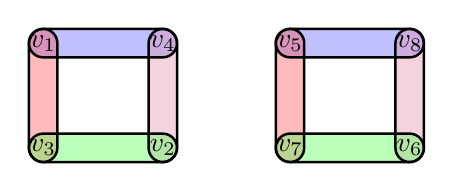
\begin{tikzpicture}[x=0.95cm,y=0.95cm]
  \fill[blue!65, fill opacity=0.38] (0.000,1.590) arc[start angle=90.00, end angle=270.00, radius=0.19] -- (1.600,1.210) arc[start angle=-90.00, end angle=90.00, radius=0.19] -- cycle;
  \fill[red!70, fill opacity=0.38] (-0.190,0.000) arc[start angle=180.00, end angle=360.00, radius=0.19] -- (0.190,1.400) arc[start angle=0.00, end angle=180.00, radius=0.19] -- cycle;
  \fill[purple!45, fill opacity=0.38] (1.410,0.000) arc[start angle=-180.00, end angle=-0.00, radius=0.19] -- (1.790,1.400) arc[start angle=-0.00, end angle=180.00, radius=0.19] -- cycle;
  \fill[green!70, fill opacity=0.38] (0.000,0.190) arc[start angle=90.00, end angle=270.00, radius=0.19] -- (1.600,-0.190) arc[start angle=-90.00, end angle=90.00, radius=0.19] -- cycle;
  \fill[blue!65, fill opacity=0.38] (3.300,1.590) arc[start angle=90.00, end angle=270.00, radius=0.19] -- (4.900,1.210) arc[start angle=-90.00, end angle=90.00, radius=0.19] -- cycle;
  \fill[red!70, fill opacity=0.38] (3.110,0.000) arc[start angle=-180.00, end angle=-0.00, radius=0.19] -- (3.490,1.400) arc[start angle=-0.00, end angle=180.00, radius=0.19] -- cycle;
  \fill[purple!45, fill opacity=0.38] (4.710,0.000) arc[start angle=-180.00, end angle=-0.00, radius=0.19] -- (5.090,1.400) arc[start angle=-0.00, end angle=180.00, radius=0.19] -- cycle;
  \fill[green!70, fill opacity=0.38] (3.300,0.190) arc[start angle=90.00, end angle=270.00, radius=0.19] -- (4.900,-0.190) arc[start angle=-90.00, end angle=90.00, radius=0.19] -- cycle;
  \draw[black, line width=0.9pt] (0.000,1.590) arc[start angle=90.00, end angle=270.00, radius=0.19] -- (1.600,1.210) arc[start angle=-90.00, end angle=90.00, radius=0.19] -- cycle;
  \draw[black, line width=0.9pt] (-0.190,0.000) arc[start angle=180.00, end angle=360.00, radius=0.19] -- (0.190,1.400) arc[start angle=0.00, end angle=180.00, radius=0.19] -- cycle;
  \draw[black, line width=0.9pt] (1.410,0.000) arc[start angle=-180.00, end angle=-0.00, radius=0.19] -- (1.790,1.400) arc[start angle=-0.00, end angle=180.00, radius=0.19] -- cycle;
  \draw[black, line width=0.9pt] (0.000,0.190) arc[start angle=90.00, end angle=270.00, radius=0.19] -- (1.600,-0.190) arc[start angle=-90.00, end angle=90.00, radius=0.19] -- cycle;
  \draw[black, line width=0.9pt] (3.300,1.590) arc[start angle=90.00, end angle=270.00, radius=0.19] -- (4.900,1.210) arc[start angle=-90.00, end angle=90.00, radius=0.19] -- cycle;
  \draw[black, line width=0.9pt] (3.110,0.000) arc[start angle=-180.00, end angle=-0.00, radius=0.19] -- (3.490,1.400) arc[start angle=-0.00, end angle=180.00, radius=0.19] -- cycle;
  \draw[black, line width=0.9pt] (4.710,0.000) arc[start angle=-180.00, end angle=-0.00, radius=0.19] -- (5.090,1.400) arc[start angle=-0.00, end angle=180.00, radius=0.19] -- cycle;
  \draw[black, line width=0.9pt] (3.300,0.190) arc[start angle=90.00, end angle=270.00, radius=0.19] -- (4.900,-0.190) arc[start angle=-90.00, end angle=90.00, radius=0.19] -- cycle;
  \node[inner sep=0pt] at (0.000,1.400) {$v_{1}$};
  \node[inner sep=0pt] at (1.600,1.400) {$v_{4}$};
  \node[inner sep=0pt] at (0.000,0.000) {$v_{3}$};
  \node[inner sep=0pt] at (1.600,0.000) {$v_{2}$};
  \node[inner sep=0pt] at (3.300,1.400) {$v_{5}$};
  \node[inner sep=0pt] at (4.900,1.400) {$v_{8}$};
  \node[inner sep=0pt] at (3.300,0.000) {$v_{7}$};
  \node[inner sep=0pt] at (4.900,0.000) {$v_{6}$};
\end{tikzpicture}
\caption{$f_2$}\end{subfigure}\hfill
\begin{subfigure}{0.5\linewidth}\centering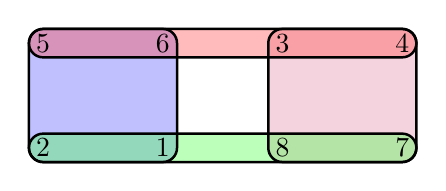
\begin{tikzpicture}[x=0.95cm,y=0.95cm]
  \fill[blue!65, fill opacity=0.38] (-0.190,0.000) arc[start angle=180.00, end angle=270.00, radius=0.19] -- (1.600,-0.190) arc[start angle=-90.00, end angle=-0.00, radius=0.19] -- (1.790,1.400) arc[start angle=-0.00, end angle=90.00, radius=0.19] -- (0.000,1.590) arc[start angle=90.00, end angle=180.00, radius=0.19] -- cycle;
  \fill[purple!45, fill opacity=0.38] (3.010,0.000) arc[start angle=-180.00, end angle=-90.00, radius=0.19] -- (4.800,-0.190) arc[start angle=-90.00, end angle=-0.00, radius=0.19] -- (4.990,1.400) arc[start angle=-0.00, end angle=90.00, radius=0.19] -- (3.200,1.590) arc[start angle=90.00, end angle=180.00, radius=0.19] -- cycle;
  \fill[red!70, fill opacity=0.38] (0.000,1.590) arc[start angle=90.00, end angle=270.00, radius=0.19] -- (4.800,1.210) arc[start angle=-90.00, end angle=90.00, radius=0.19] -- cycle;
  \fill[green!70, fill opacity=0.38] (0.000,0.190) arc[start angle=90.00, end angle=270.00, radius=0.19] -- (4.800,-0.190) arc[start angle=-90.00, end angle=90.00, radius=0.19] -- cycle;
  \draw[black, line width=0.9pt] (-0.190,0.000) arc[start angle=180.00, end angle=270.00, radius=0.19] -- (1.600,-0.190) arc[start angle=-90.00, end angle=-0.00, radius=0.19] -- (1.790,1.400) arc[start angle=-0.00, end angle=90.00, radius=0.19] -- (0.000,1.590) arc[start angle=90.00, end angle=180.00, radius=0.19] -- cycle;
  \draw[black, line width=0.9pt] (3.010,0.000) arc[start angle=-180.00, end angle=-90.00, radius=0.19] -- (4.800,-0.190) arc[start angle=-90.00, end angle=-0.00, radius=0.19] -- (4.990,1.400) arc[start angle=-0.00, end angle=90.00, radius=0.19] -- (3.200,1.590) arc[start angle=90.00, end angle=180.00, radius=0.19] -- cycle;
  \draw[black, line width=0.9pt] (0.000,1.590) arc[start angle=90.00, end angle=270.00, radius=0.19] -- (4.800,1.210) arc[start angle=-90.00, end angle=90.00, radius=0.19] -- cycle;
  \draw[black, line width=0.9pt] (0.000,0.190) arc[start angle=90.00, end angle=270.00, radius=0.19] -- (4.800,-0.190) arc[start angle=-90.00, end angle=90.00, radius=0.19] -- cycle;
  \node[inner sep=0pt] at (0.000,1.400) {$5$};
  \node[inner sep=0pt] at (1.600,1.400) {$6$};
  \node[inner sep=0pt] at (3.200,1.400) {$3$};
  \node[inner sep=0pt] at (4.800,1.400) {$4$};
  \node[inner sep=0pt] at (0.000,0.000) {$2$};
  \node[inner sep=0pt] at (1.600,0.000) {$1$};
  \node[inner sep=0pt] at (3.200,0.000) {$8$};
  \node[inner sep=0pt] at (4.800,0.000) {$7$};
\end{tikzpicture}
\caption{$g_2$}\end{subfigure}
\caption{Hypergraphs $f_2$ and $g_2$ in the $\GK$-family.}
\end{figure}

\subsection{$\TK$-family}

Takata denoted a class of recursively defined hypergraphs and their transversals as \emph{alternating trees} as well. We will address them as $\TK$-family. The set of hypergraphs $S_k\in\TK$ is defined recursively as follows:
\[
S_0=v_1,\quad S_1=(v_1\vee v_2)\wedge(v_3\vee v_4).
\]
For $k\geq 2$, $S_k$ is constructed as:
\[
S_k=(A\vee B)\wedge(C\vee D),
\]
where $A,B,C,D$ are vertex-disjoint copies of $S_{k-1}$.

The transversal hypergraph of $S_k$, denoted $r_k$, is defined recursively as follows:
\[
r_0=v_1,\quad r_1=(v_1\wedge v_2)\vee(v_3\wedge v_4).
\]
For $k\geq 2$, $r_k$ is constructed as:
\[
r_k=(A_1\wedge A_2)\vee(A_3\wedge A_4),
\]
where $A_i$, $i=1,\dots,4$ are vertex-disjoint copies of $r_{k-1}$.

\subsection{Combined Alternating Trees}

Hertel defined the combined alternating trees recursively as follows:
\[
\Gamma_0=\{v\},\quad\Gamma_i=\begin{cases}A\wedge B&\text{if }i\text{ odd},\\A\vee B&\text{if }i\text{ even.}\end{cases}
\]
where $A$ and $B$ are vertex-disjoint copies of $\Gamma_{i-1}$, and $\{v\}$ represents a hypergraph with a single edge containing one vertex. \cite{Her04}

The alternating tree $\Gamma_i$ corresponds to a hypergraph $H_i$ with $2^i$ vertices, forming a binary tree of height $i$, where each leaf represents a distinct vertex. They correspond to specific hypergraph families: $\GK$-family for odd $i$, and $\TK$-family for even $i$.

Denoting the set of edges of hypergraphs $H_i$ as $E_i$, we have:
\[
|E_0|=1,\quad|E_i|=\begin{cases}|E_{i-1}|^2&\text{if }i\text{ is odd,}\\2\times|E_{i-1}|&\text{if }i\text{ is even,}\end{cases}\qquad|E_i|=2^{2^{i/2}-1}\text{ for even }i.
\]

Similarly, denoting the set of transversals (edges in $\Tr(H_i)$) as $E_i'$, when $\Tr(H)$ is generated by $\Gamma_i$:
\[
|E_0'|=1,\quad|E_i'|=\begin{cases}2\times|E_{i-1}'|&\text{if }i\text{ is odd,}\\|E_{i-1}'|^2&\text{if }i\text{ is even,}\end{cases}\qquad|E_i'|=2^{2^{i/2+1}-2}\text{ for even }i.
\]
These are \leanref{card_alt_succ}, \leanref{card_coalt_succ} and \leanref{alt_counts}. The 2024 edition printed the two cases of each recurrence exchanged \leanref{printed_recurrence_fails} and the closed forms $2^{2^{(i/2)-1}}$ and $2^{(i/2)-1}$, which fail at $i=4$.

To generate the hypergraph $g_2$ in the $\GK$-family, $\vee$ (\emph{union}) of the edges in $\Gamma_3$ are considered. Similarly, the hypergraph $f_2$ in the $\GK$-family is generated by taking $\wedge$ (\emph{join}) of the edges in $\Gamma_3$, with edges in $f_2$ and $g_2$ representing the resulting vertex sets.

Gurvich first characterized these alternating trees by properties of their primal graphs in the 70's \cite{Gc77}. Hertel identified the alternating trees as the \emph{read-once} hypergraphs \cite{Her04}. They are also called exact-transversal hypergraphs or \emph{xt}-hypergraphs \cite{Eit94}. In Boolean terms, they are known as read-once functions. \cite{GMR06} shows that there is a one-to-one correspondence between read-once Boolean functions and read-once hypergraphs.

\begin{figure}[h]
\centering
\begin{forest}
for tree={draw, font=\tiny, inner sep=2pt, l sep=6mm, s sep=4mm, edge={thin}}
[$\wedge$
  [$\vee$ [$\wedge$ [$v_1$] [$v_2$]] [$\wedge$ [$v_3$] [$v_4$]]]
  [$\vee$ [$\wedge$ [$v_5$] [$v_6$]] [$\wedge$ [$v_7$] [$v_8$]]]
]
\end{forest}
\caption{Alternating Tree $g_2$ in $\GK$ family}
\end{figure}

\section{Frequency Bound on Alternating Families}

\subsection{Bound on $\GK$-family}

Let $E(f_k),E(g_k)$ denote the sets of hyperedges of $f_k$, and $g_k$. It naturally follows that, $|E(f_1)|=2,|E(f_2)|=2^3,\dots,|E(f_{k+1})|=2\cdot|E(f_k)|^2$. This leads to, $|(f_k)|=2^{2^k-1}$ for $k=1,2,\dots$ \leanref{alt_counts}.

The frequency $\epsilon(f_k)$ for each vertex $v_i$ in each $f_k$ is uniform, and since $|e|=2^{k-1},\forall e\in E(f_k)$, we get that $\epsilon_k=2^{-k}$ \leanref{alt_shape}.

Similarly, we get that $|E(g_1)|=1,|E(g_2)|=2^2,\dots,|E(g_{k+1})|=(2\cdot|E(g_k)|)^2$, leading to $|E(g_k)|=\frac{1}{2}\cdot|f_k|=2^{2^k-2}$ for $k=1,2,\dots$. Since $|e|=2^k,\forall e\in E(g_k)$, each vertex $v_i$ occurs in $g_k$ with the uniform frequency $\epsilon(g_k)=2^{1-k}$.

Then, we get $\max\{\epsilon(f_k),\epsilon(g_k)\}=2^{1-k}\leq\frac{2}{\log_2(|E(f_k)|+|E(g_k)|)}=\frac{2}{2^k+\log_2(3/4)}$.

Clearly, $f_k$ is comprised of $2^k$ distinct vertices and they form a binary recursive tree of height $k$, where each leaf is a distinct vertex. We join two vertex-disjoint copies of $f_{k-1}$ to construct $f_k$.

In current literature, is not clear how the frequency at the top level, i.e. at the level of the original input hypergraphs $f_k$ and $g_k$ influences the behavior of \FKA{} at the lower levels of the recursion.

\subsection{Frequency Bound on $\TK$-family of Hypergraphs}

Let $E(S_i)$ and $E(r_i)$ denote the sets of hyperedges of $S_i$ and its transversal hypergraph $r_i$. For the $\TK$-family, the size of $S_i$ grows as $|E(S_1)|=4$, $|E(S_2)|=(2\cdot|E(S_1)|)^2$, leading to $|E(S_i)|=2^{2(2^i-1)}$ for $i=1,2,\dots$.

The frequency $\epsilon(S_i)$ for each vertex in $S_i$ is uniform. Since the size of each hyperedge $|e|=2^i$ and $|e|=|V(S_i)|\cdot\epsilon(S_i)$ for any $e\in E(S_i)$, we get $\epsilon(S_i)=2^{-i}$ \leanref{alt_shape}.

For the transversal hypergraph $r_i$, we observe similar frequency behavior. The size of each edge in $E(r_i)$ matches that in $E(S_i)$. Using the same argument, $\epsilon(r_i)=2^{-i}$. Combining these, we get:
\[
\epsilon(S_i)=2^{-i}\leq\frac{2}{\log_2(|E(S_i)|+|E(r_i)|)}.
\]
Since $|E(S_i)|=2^{2(2^i-1)}$ and $|E(r_i)|=2^{2^i-1}$, the frequency bound becomes:
\[
\epsilon(S_i)\leq\frac{2}{\log_2(2^{2(2^i-1)}+2^{2^i-1})}.
\]
Both families of hypergraphs, despite having slightly different structure, attains the bound presented by \cite{FK96}.

\section{Read-Once Hypergraphs}\label{sec:read-once}

\begin{definition}
A hypergraph $H$ is called \emph{read-once} if it can be represented by an expression using the operations of \emph{join} $(\wedge)$, and \emph{union} $(\vee)$, in which each vertex appears exactly once. Such an expression is called a \emph{read-once expression}.
\end{definition}

\cite{CH11}

\begin{example}
Consider the Boolean function
\[
f_0=(v_1\wedge v_6)\vee(v_3\wedge v_5\wedge v_6)\vee(v_2\wedge v_4)\vee(v_2\wedge v_7).
\]
This is a read-once hypergraph since it can be factored into the read-once expression
\[
f_0=(v_6\wedge(v_1\vee(v_3\wedge v_5)))\vee(v_2\wedge(v_4\vee v_7),
\]
which is a read-once expression.
\end{example}

Read-once hypergraph have been studied since the 60's \cite{Che67} and Hayes \cite{Hay75}. Gurvich first characterized them in \cite{Gc77} as the following: A hypergraph $H=(V,E)$ is \emph{read-once} if and only if:
\begin{itemize}
\item $H$ is conformal.
\item The primal graph $G(H)$ of $H$ has no induced $P_4$
\end{itemize}
The class of graphs who don't contain any induced $P_4$ are called cographs. \cite{CLB81}

\subsection{Primal Graphs of Read-Once Hypergraphs}

Primal graphs of conformal hypergraphs often belong to well-known graph classes, such as perfect graphs. One such class of perfect graphs are cographs \ref{sec:read-once}. Other class of perfect graphs who are primal graphs of hypergraphs include chordal graphs, chordal bipartite graphs etc. These graph classes help characterize the structures and symmetries of several families of $k$-uniform hypergraphs.

\begin{definition}\label{def:chordal}
A graph $G$ is called \emph{chordal} (or \emph{triangulated}) if every cycle of length at least four has a \emph{chord}, where a chord is an edge $e\in E(G)$ that is not part of the cycle but connects two non-consecutive vertices in the cycle.
\end{definition}

\begin{definition}
A hypergraph $H=(V,E)$ is \emph{$\alpha$-acyclic} if it is conformal and its primal graph $G(H)$ is chordal.
\end{definition}

\begin{definition}
A bipartite graph $G=(U\cup W,E)$ is called \emph{chordal bipartite} if every cycle of length at least six has a chord.
\end{definition}

Primal graphs of read-once hypergraphs are called complement reducible graphs or \emph{cographs} \ref{sec:read-once}.

Cographs have been characterized independently by \cite{CLB81}, \cite{Gc77}, \cite{KLN+93}. We present the following to examine the structure of cographs.

\begin{definition}
A \emph{cograph} () can also be defined recursively as follows: \cite{Cam22}
\begin{enumerate}
\item A single vertex $v$ is a cograph.
\item The union $(\vee)$ of disjoint cographs is a cograph.
\item The join $(\wedge)$ of disjoint cographs is a cograph.
\item The complement $G^c$ of a cograph $G$ is a cograph.
\end{enumerate}
\end{definition}

\begin{lemma}
If $G$ is a cograph with more than one vertex, then either $G$ or its complement $G^C$ is disconnected. \cite{CLB81}
\end{lemma}

The recursive building of a cograph $G$ from a single vertex can be represented by a rooted tree $T$, denoted the \emph{cotree}, defined as:
\begin{enumerate}
\item The leaf nodes of $T$ are labeled by the vertices of $G$.
\item Each non-leaf vertex has at least two children.
\item All non-leaf vertices of $T$ are labelled either by $\vee$ or $\wedge$.
\item If $G$ is formed from the disjoint cographs $G_1,G_2,\dots,G_k$ $(k>1)$, then the root $r$ of $T$ has as its children the roots of the trees of $G_1,G_2,\dots,G_k$.
\item The root $r$ is labeled $\vee$ if $G$ is formed by the union, and labeled $\wedge$ if $G$ is formed by the join rule. \refstepcounter{equation}(\theequation)
\item On every path from the root to a leaf node in $T$, the labels of the internal nodes alternate between $\vee$ and $\wedge$.
\end{enumerate}

The root of the cotree is labeled $\vee$ if $G$ is disconnected and labeled $\wedge$ if $G$ is connected. An internal node is labeled $\vee$ if its parent is labeled $\wedge$, and vice versa.

A hypergraph, defined using the operations of join $(\wedge)$ and union $(\vee)$, can be represented as a rooted parse tree. The leaves of this tree are labeled by the vertices $\{v_1,v_2,\dots,v_n\}$, while the internal nodes are labeled with the operations $\wedge$ and $\vee$. For a read-once hypergraph, each vertex appears exactly once as a leaf, with a unique path from the root to the vertex.

The cotree of a $P_4$-free graph closely resembles the parse tree of a read-once hypergraph. If the hypergraph is read-once, its parse tree coincides with the cotree of its primal graph, which is a cograph. Conversely, a cotree always generates a read-once hypergraph.

\begin{theorem}
A graph $G$ has a cotree representation if and only if $G$ is a cograph. In this case, the cotree representation is unique.
\end{theorem}

\cite{CLB81}

Given the correspondence between the parse-tree and cotree representation of a hypergraph, we make the following observation:

\begin{observation}[\leanref{primalAdj_alt}]
The alternating tree presented in \cite{Her04} (\ref{sec:alternating}) is a cotree representation of the $\GK$-family and of the $\TK$-family: for every $i$, two vertices are adjacent in the primal graph of $\Gamma_i$ (resp.\ $\Gamma_i'$) exactly when they are adjacent in the cograph of the alternating tree.
\end{observation}

\subsection{Automorphism Structure of Read-Once Hypergraphs}

\begin{definition}
Let $H=(V,E)$ be a hypergraph and $S\subseteq V$. The \emph{open neighborhood} of $S$, denoted by $N(S)$, is the set of vertices adjacent to $S$, excluding $S$, i.e.,
\[
N(S)=\{v\in V\mid\exists e\in E,v\in e,S\cap e\neq\emptyset,v\notin S\}.
\]
The \emph{closed neighborhood} of $S$, denoted by $N[S]$, is the union of the open neighborhood and $S$, i.e.,
\[
N[S]=N(S)\cup S.
\]
For a single vertex $v\in V$, we write $N(v)$ for $N(\{v\})$ and $N[v]$ for $N[\{v\}]$.
\end{definition}

\begin{definition}
Two distinct vertices $u,v\in V$ of a hypergraph $H$ are called:
\begin{itemize}
\item \emph{False twins} if $N(u)=N(v)$,
\item \emph{True twins} if $N[u]=N[v]$, in which case $u$ and $v$ are adjacent.
\end{itemize}
\end{definition}

More generally, two vertices are said to be \emph{twins} if they are either false twins or true twins. Being twins in a graph is an equivalence relation. Twins in the same orbit of the automorphism group are in the same equivalence class.

Consider a hypergraph with vertices $\{v_1,v_2,v_3,v_4\}$ and hyperedges $\{\{v_1,v_2\},\{v_2,v_3,v_4\},\{v_1,v_3\}\}$. The neighborhoods are $N(v_1)=\{v_2,v_3\}$, $N(v_2)=\{v_1,v_3,v_4\}$, $N(v_3)=\{v_1,v_2,v_4\}$, and $N(v_4)=\{v_2,v_3\}$. Vertices $v_2$ and $v_3$ are true twins because their closed neighborhoods are identical, $N[v_2]=N[v_3]=\{v_1,v_2,v_3,v_4\}$. In contrast, $v_1$ and $v_4$ are false twins because their open neighborhoods are the same, $N(v_1)=N(v_4)=\{v_2,v_3\}$.

Cographs belong to the class of distance-hereditary graphs. (The 2024 edition included chordal graphs; the gem, a path $v_1v_2v_3v_4$ with a fifth vertex adjacent to all four, is chordal and not distance-hereditary: \leanref{gem_chordal_four}, \leanref{gem_chordal_five}, \leanref{gem_not_distance_hereditary}.)

\begin{definition}
A graph $G=(V,E)$ is called \emph{distance hereditary} if, for every connected induced subgraph $G'=(V',E')$ of $G$, the distance (\ref{def:distance}) between any two vertices $u,v\in V'$ in $G'$ is the same as their distance in $G$. Formally, $G$ is distance hereditary if, for every connected induced subgraph $G'$, $d_{G'}(u,v)=d_G(u,v)$ for all $u,v\in V'$.
\end{definition}

\begin{lemma}[\leanref{twins_mem_aut_cliques}]\label{lem:twins-permute}
Let $G=(V,E)$ be a graph, $H$ its clique hypergraph, and $\Tr(H)$ its transversal hypergraph. If $u,v\in V$ are twin vertices in $G$, then $u$ and $v$ permute in both $H$ and $\Tr(H)$. \cite{Tim13}
\end{lemma}

\begin{proof}
The transposition $(u\,v)$ is an automorphism of $G$: it fixes every vertex other than $u,v$, and twins have the same neighbours outside $\{u,v\}$ \leanref{swap_isAut_of_twins}. A graph automorphism maps maximal cliques to maximal cliques, so $(u\,v)\in\Aut(H)$, and $\Aut(H)\le\Aut(\Tr(H))$ \leanref{aut_le_aut_tr}. No hypothesis on $G$ is needed.
\end{proof}

The 2024 edition assumed $G$ distance-hereditary and $H$ conformal, and its proof, kept below for the record, is incorrect: a stable set containing $u$ need not contain its false twin $v$.

\begin{proof}[Proof printed in 2024]
If $u$ and $v$ are true twins in $G$, they share identical neighborhoods and are adjacent. Any maximal clique in $G$ containing $u$ must also contain $v$. In $H$, this ensures $u$ and $v$ co-appear in every hyperedge corresponding to a maximal clique, and thus $u$ and $v$ permute in $H$. Similarly, if $u$ and $v$ are false twins, they share identical neighborhoods but are not adjacent. Any stable set in $G$ containing $u$ must also contain $v$. Consequently, in $\Tr(H)$, $u$ and $v$ co-appear in every hyperedge corresponding to a stable set, ensuring their permutation in $\Tr(H)$.

For conformal $H$, each maximal clique in $G$ directly corresponds to a hyperedge in $H$, preserving the structural symmetry of $u$ and $v$. Hence, $u$ and $v$ permute in both $H$ and $\Tr(H)$.
\end{proof}

If $H$ is non-conformal, the mapping of maximal cliques or stable sets to hyperedges may not hold, potentially breaking the symmetry. Therefore, we see that the presence of twins in read-once hypergraphs means they will permute in the primal graph, thus creating localized symmetries in the hypergraphs.

\begin{lemma}[\leanref{twins_map}]\label{lem:twins-map}
Let $H=(V,E)$ be a hypergraph and $\phi:V\to V$ be an automorphism of $H$. If $u_1,u_2\in V$ are true twins or $v_1,v_2\in V$ are false twins in $H$, then $\phi(u_1),\phi(u_2)$ are true twins, and $\phi(v_1),\phi(v_2)$ are false twins in $H$.
\end{lemma}

\begin{proof}
True twins $u_1$ and $u_2$ satisfy $N[u_1]=N[u_2]$, meaning they are adjacent and share the same neighbors. Since $\phi$ is an automorphism preserving adjacency, $\phi(u_1)$ and $\phi(u_2)$ are also adjacent, and $\phi(N[u_1])=N[\phi(u_1)]$, $\phi(N[u_2])=N[\phi(u_2)]$. Thus, $N[\phi(u_1)]=N[\phi(u_2)]$, confirming $\phi(u_1)$ and $\phi(u_2)$ are true twins.

False twins $v_1$ and $v_2$ satisfy $N(v_1)=N(v_2)$, sharing neighbors but not being adjacent. As $\phi$ preserves non-adjacency, $\phi(v_1)$ and $\phi(v_2)$ are also non-adjacent, with $\phi(N(v_1))=N(\phi(v_1))$, $\phi(N(v_2))=N(\phi(v_2))$. Hence, $N(\phi(v_1))=N(\phi(v_2))$, confirming $\phi(v_1)$ and $\phi(v_2)$ are false twins.

Thus, $\phi$ maps true twins to true twins and false twins to false twins in $H$ i.e. twin-classes get mapped to other twin-classes.
\end{proof}

For a graph $G$, permuting twin vertices while fixing all other vertices is an automorphism of $G$. Consequently, the automorphism group of $G$ contains a normal subgroup that is the direct product of symmetric groups corresponding to the twin classes.

\begin{proposition}\label{prop:cameron}
Let $G$ be a cograph. The automorphism group of $G$ can be constructed from the trivial group using direct product (\ref{sec:symmetries}) and wreath product with a symmetric group. \cite{Cam22}
\end{proposition}

A cograph hypergraph can be built from the single-vertex hypergraph using operations of complement and disjoint union. Complementation does not alter the automorphism group. If $H$ is the disjoint union of $m_1$ copies of $H_1$, $m_2$ copies of $H_2$, ..., $m_r$ copies of $H_r$, then the automorphism group of $H$ is given by:
\[
\Aut(H)=(\Aut(H_1)\wr S_{m_1})\times\dots\times(\Aut(H_r)\wr S_{m_r})
\]
